% Constructed and checked from the problem; not a geometric proof.
\documentclass[tikz,border=8pt]{standalone}
\begin{document}
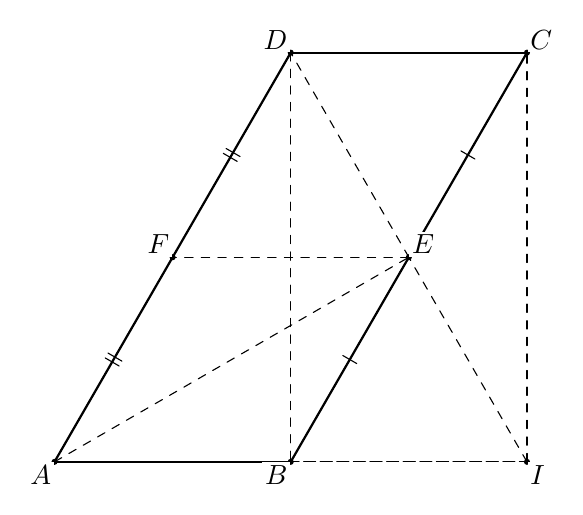
\begin{tikzpicture}[scale=1,line cap=round,line join=round]
\coordinate (p0) at (0,0);
\coordinate (p1) at (3,0);
\coordinate (p2) at (6,5.1961524);
\coordinate (p3) at (3,5.1961524);
\coordinate (p4) at (4.5,2.5980762);
\coordinate (p5) at (1.5,2.5980762);
\coordinate (p6) at (6,0);
\draw[thick] (p0) -- (p1);
\draw[thick] (p1) -- (p2);
\draw[thick] (p2) -- (p3);
\draw[thick] (p3) -- (p0);
\draw[dashed] (p0) -- (p6);
\draw[dashed] (p1) -- (p4);
\draw[dashed] (p4) -- (p5);
\draw[dashed] (p5) -- (p0);
\draw[dashed] (p6) -- (p4);
\draw[dashed] (p1) -- (p6);
\draw[dashed] (p6) -- (p2);
\draw[dashed] (p3) -- (p1);
\draw[dashed] (p0) -- (p4);
\draw[dashed] (p4) -- (p3);
\draw (3.6616654,1.3500381) -- (3.8383346,1.2480381);
\draw (5.1616654,3.9481143) -- (5.3383346,3.8461143);
\draw (0.6438154,1.319121) -- (0.8204846,1.217121);
\draw (0.6795154,1.3809552) -- (0.8561846,1.2789552);
\draw (2.1438154,3.9171972) -- (2.3204846,3.8151972);
\draw (2.1795154,3.9790314) -- (2.3561846,3.8770314);
\fill (p0) circle (1.1pt) node[fill=white,inner sep=1pt,below left] {$A$};
\fill (p1) circle (1.1pt) node[fill=white,inner sep=1pt,below left] {$B$};
\fill (p2) circle (1.1pt) node[fill=white,inner sep=1pt,above right] {$C$};
\fill (p3) circle (1.1pt) node[fill=white,inner sep=1pt,above left] {$D$};
\fill (p4) circle (1.1pt) node[fill=white,inner sep=1pt,above right] {$E$};
\fill (p5) circle (1.1pt) node[fill=white,inner sep=1pt,above left] {$F$};
\fill (p6) circle (1.1pt) node[fill=white,inner sep=1pt,below right] {$I$};
\end{tikzpicture}
\end{document}
